\documentclass[twoside]{book}

% Packages required by doxygen
\usepackage{fixltx2e}
\usepackage{calc}
\usepackage{doxygen}
\usepackage[export]{adjustbox} % also loads graphicx
\usepackage{graphicx}
\usepackage[utf8]{inputenc}
\usepackage{makeidx}
\usepackage{multicol}
\usepackage{multirow}
\PassOptionsToPackage{warn}{textcomp}
\usepackage{textcomp}
\usepackage[nointegrals]{wasysym}
\usepackage[table]{xcolor}

% Font selection
\usepackage[T1]{fontenc}
\usepackage[scaled=.90]{helvet}
\usepackage{courier}
\usepackage{amssymb}
\usepackage{sectsty}
\renewcommand{\familydefault}{\sfdefault}
\allsectionsfont{%
  \fontseries{bc}\selectfont%
  \color{darkgray}%
}
\renewcommand{\DoxyLabelFont}{%
  \fontseries{bc}\selectfont%
  \color{darkgray}%
}
\newcommand{\+}{\discretionary{\mbox{\scriptsize$\hookleftarrow$}}{}{}}

% Page & text layout
\usepackage{geometry}
\geometry{%
  a4paper,%
  top=2.5cm,%
  bottom=2.5cm,%
  left=2.5cm,%
  right=2.5cm%
}
\tolerance=750
\hfuzz=15pt
\hbadness=750
\setlength{\emergencystretch}{15pt}
\setlength{\parindent}{0cm}
\setlength{\parskip}{3ex plus 2ex minus 2ex}
\makeatletter
\renewcommand{\paragraph}{%
  \@startsection{paragraph}{4}{0ex}{-1.0ex}{1.0ex}{%
    \normalfont\normalsize\bfseries\SS@parafont%
  }%
}
\renewcommand{\subparagraph}{%
  \@startsection{subparagraph}{5}{0ex}{-1.0ex}{1.0ex}{%
    \normalfont\normalsize\bfseries\SS@subparafont%
  }%
}
\makeatother

% Headers & footers
\usepackage{fancyhdr}
\pagestyle{fancyplain}
\fancyhead[LE]{\fancyplain{}{\bfseries\thepage}}
\fancyhead[CE]{\fancyplain{}{}}
\fancyhead[RE]{\fancyplain{}{\bfseries\leftmark}}
\fancyhead[LO]{\fancyplain{}{\bfseries\rightmark}}
\fancyhead[CO]{\fancyplain{}{}}
\fancyhead[RO]{\fancyplain{}{\bfseries\thepage}}
\fancyfoot[LE]{\fancyplain{}{}}
\fancyfoot[CE]{\fancyplain{}{}}
\fancyfoot[RE]{\fancyplain{}{\bfseries\scriptsize Generated by Doxygen }}
\fancyfoot[LO]{\fancyplain{}{\bfseries\scriptsize Generated by Doxygen }}
\fancyfoot[CO]{\fancyplain{}{}}
\fancyfoot[RO]{\fancyplain{}{}}
\renewcommand{\footrulewidth}{0.4pt}
\renewcommand{\chaptermark}[1]{%
  \markboth{#1}{}%
}
\renewcommand{\sectionmark}[1]{%
  \markright{\thesection\ #1}%
}

% Indices & bibliography
\usepackage{natbib}
\usepackage[titles]{tocloft}
\setcounter{tocdepth}{3}
\setcounter{secnumdepth}{5}
\makeindex

% Hyperlinks (required, but should be loaded last)
\usepackage{ifpdf}
\ifpdf
  \usepackage[pdftex,pagebackref=true]{hyperref}
\else
  \usepackage[ps2pdf,pagebackref=true]{hyperref}
\fi
\hypersetup{%
  colorlinks=true,%
  linkcolor=blue,%
  citecolor=blue,%
  unicode%
}

% Custom commands
\newcommand{\clearemptydoublepage}{%
  \newpage{\pagestyle{empty}\cleardoublepage}%
}

\usepackage{caption}
\captionsetup{labelsep=space,justification=centering,font={bf},singlelinecheck=off,skip=4pt,position=top}

%===== C O N T E N T S =====

\begin{document}

% Titlepage & ToC
\hypersetup{pageanchor=false,
             bookmarksnumbered=true,
             pdfencoding=unicode
            }
\pagenumbering{roman}
\begin{titlepage}
\vspace*{7cm}
\begin{center}%
{\Large Monocular Visual Odometry \\[1ex]\large 1.\+0 }\\
\vspace*{1cm}
{\large Generated by Doxygen 1.8.11}\\
\end{center}
\end{titlepage}
\clearemptydoublepage
\tableofcontents
\clearemptydoublepage
\pagenumbering{arabic}
\hypersetup{pageanchor=true}

%--- Begin generated contents ---
\chapter{Monocular Visual Odometry}
\label{index}\hypertarget{index}{}\subsection*{Overview}

This is a personal project with the objective of developing a custom implementation of Monocular Visual Odometry. I hope to contribute to this library fairly regularly. I will also be generating Doxygen documentation eventually.

\subsection*{Note }

This library is just a straightforward implementation at the moment. I plan to optimize it further and even use it for basic S\+L\+AM, down the line.

\subsection*{Inputs }

I will be using the K\+I\+T\+TI Odometry dataset. The ground truth poses will be used to compute absolute scale (seeing as I don\textquotesingle{}t have access to actual speedometer readings \+:P). I will be considering the folder structure to be similar to the K\+I\+T\+T\+I\+\_\+\+VO dataset. So if you want to use the code for yourself, you just need to change the base path as long as the internal folder structure is the same.


\begin{DoxyCode}
1 Path to folder
2 +-- KITTI\_VO/
3 |   +-- poses/
4 |       +-- ground truth .txt files starting with 00.txt
5 |   +-- sequences/
6 |       +-- Sequence ID based folders (00/)
7 |           +-- image\_2/
8 |               +-- video frames in .png format, starting with 000000.png
9 |           +-- image\_3/
10 |               +-- video frames in .png format, starting with 000000.png
11 |           +-- calib.txt
12 |           +-- times.txt
\end{DoxyCode}


\subsection*{Todo (09/2/2018) }


\begin{DoxyEnumerate}
\item Test accuracy of Pose decomposition \& optimize function
\item Move Window generation to class and add destructor to close windows after end of execution.
\item Add P\+CL support for R\+A\+N\+S\+AC.
\item Convert to Eigen (Painful but necessary)
\end{DoxyEnumerate}

Example code on how to use the library will be updated in the cpp file src/main.\+cc.

\subsection*{How to build and run the demo}


\begin{DoxyItemize}
\item To build and run demo\+: Update path to dataset in main.\+cc. 
\begin{DoxyCode}
1 mkdir build
2 cd build
3 cmake ..
4 make
5 ./vo
\end{DoxyCode}
 To use these functions in your own code. Add the include directory path to the compiler debugging. Include to the start of your code and call the functions\+:
\item To use the feature tracking and refinement library\+: 
\begin{DoxyCode}
1 #include "FeatTrack.hpp" 
\end{DoxyCode}

\item To use the egomotion estimation library\+: 
\begin{DoxyCode}
1 #include "epipolar.hpp" 
\end{DoxyCode}

\end{DoxyItemize}

\subsection*{License}

M\+IT License

Copyright (c) 2018 Yash Manian

Permission is hereby granted, free of charge, to any person obtaining a copy of this software and associated documentation files (the \char`\"{}\+Software\char`\"{}), to deal in the Software without restriction, including without limitation the rights to use, copy, modify, merge, publish, distribute, sublicense, and/or sell copies of the Software, and to permit persons to whom the Software is furnished to do so, subject to the following conditions\+:

The above copyright notice and this permission notice shall be included in all copies or substantial portions of the Software.

T\+HE S\+O\+F\+T\+W\+A\+RE IS P\+R\+O\+V\+I\+D\+ED \char`\"{}\+A\+S I\+S\char`\"{}, W\+I\+T\+H\+O\+UT W\+A\+R\+R\+A\+N\+TY OF A\+NY K\+I\+ND, E\+X\+P\+R\+E\+SS OR I\+M\+P\+L\+I\+ED, I\+N\+C\+L\+U\+D\+I\+NG B\+UT N\+OT L\+I\+M\+I\+T\+ED TO T\+HE W\+A\+R\+R\+A\+N\+T\+I\+ES OF M\+E\+R\+C\+H\+A\+N\+T\+A\+B\+I\+L\+I\+TY, F\+I\+T\+N\+E\+SS F\+OR A P\+A\+R\+T\+I\+C\+U\+L\+AR P\+U\+R\+P\+O\+SE A\+ND N\+O\+N\+I\+N\+F\+R\+I\+N\+G\+E\+M\+E\+NT. IN NO E\+V\+E\+NT S\+H\+A\+LL T\+HE A\+U\+T\+H\+O\+RS OR C\+O\+P\+Y\+R\+I\+G\+HT H\+O\+L\+D\+E\+RS BE L\+I\+A\+B\+LE F\+OR A\+NY C\+L\+A\+IM, D\+A\+M\+A\+G\+ES OR O\+T\+H\+ER L\+I\+A\+B\+I\+L\+I\+TY, W\+H\+E\+T\+H\+ER IN AN A\+C\+T\+I\+ON OF C\+O\+N\+T\+R\+A\+CT, T\+O\+RT OR O\+T\+H\+E\+R\+W\+I\+SE, A\+R\+I\+S\+I\+NG F\+R\+OM, O\+UT OF OR IN C\+O\+N\+N\+E\+C\+T\+I\+ON W\+I\+TH T\+HE S\+O\+F\+T\+W\+A\+RE OR T\+HE U\+SE OR O\+T\+H\+ER D\+E\+A\+L\+I\+N\+GS IN T\+HE S\+O\+F\+T\+W\+A\+RE. 
\chapter{Hierarchical Index}
\section{Class Hierarchy}
This inheritance list is sorted roughly, but not completely, alphabetically\+:\begin{DoxyCompactList}
\item \contentsline{section}{Feat\+Track}{\pageref{class_feat_track}}{}
\item \contentsline{section}{Point\+Ops}{\pageref{class_point_ops}}{}
\begin{DoxyCompactList}
\item \contentsline{section}{epipolar}{\pageref{classepipolar}}{}
\end{DoxyCompactList}
\end{DoxyCompactList}

\chapter{Class Index}
\section{Class List}
Here are the classes, structs, unions and interfaces with brief descriptions\+:\begin{DoxyCompactList}
\item\contentsline{section}{\hyperlink{classepipolar}{epipolar} \\*Definition of the epipolar class. It contains all the functions and variables required to compute epipolar geometry }{\pageref{classepipolar}}{}
\item\contentsline{section}{\hyperlink{class_feat_track}{Feat\+Track} \\*Definition of the \hyperlink{class_feat_track}{Feat\+Track} class. It contains all the functions and variables for detection, tracking and computing homography }{\pageref{class_feat_track}}{}
\item\contentsline{section}{\hyperlink{class_point_ops}{Point\+Ops} \\*Definition of the \hyperlink{class_point_ops}{Point\+Ops} class. It contains all the functions and variables required manipulate point formats }{\pageref{class_point_ops}}{}
\end{DoxyCompactList}

\chapter{File Index}
\section{File List}
Here is a list of all documented files with brief descriptions\+:\begin{DoxyCompactList}
\item\contentsline{section}{/home/yashmanian/\+C\+P\+P/\+Monocular\+V\+O/include/\hyperlink{epipolar_8hpp}{epipolar.\+hpp} \\*Header file with definitions for class epipolar }{\pageref{epipolar_8hpp}}{}
\item\contentsline{section}{/home/yashmanian/\+C\+P\+P/\+Monocular\+V\+O/include/\hyperlink{_feat_track_8hpp}{Feat\+Track.\+hpp} \\*Header file with definitions for class \hyperlink{class_feat_track}{Feat\+Track} }{\pageref{_feat_track_8hpp}}{}
\item\contentsline{section}{/home/yashmanian/\+C\+P\+P/\+Monocular\+V\+O/include/\hyperlink{_point_ops_8hpp}{Point\+Ops.\+hpp} \\*Header file with definitions for class \hyperlink{class_point_ops}{Point\+Ops} }{\pageref{_point_ops_8hpp}}{}
\item\contentsline{section}{/home/yashmanian/\+C\+P\+P/\+Monocular\+V\+O/src/src\+Files/\hyperlink{epipolar_8cpp}{epipolar.\+cpp} \\*Function definitions for methods declared in class epipolar }{\pageref{epipolar_8cpp}}{}
\item\contentsline{section}{/home/yashmanian/\+C\+P\+P/\+Monocular\+V\+O/src/src\+Files/\hyperlink{_feat_track_8cpp}{Feat\+Track.\+cpp} \\*Function definitions for methods declared in class \hyperlink{class_feat_track}{Feat\+Track} }{\pageref{_feat_track_8cpp}}{}
\item\contentsline{section}{/home/yashmanian/\+C\+P\+P/\+Monocular\+V\+O/src/src\+Files/\hyperlink{_point_ops_8cpp}{Point\+Ops.\+cpp} \\*Function definitions for methods declared in class \hyperlink{class_point_ops}{Point\+Ops} }{\pageref{_point_ops_8cpp}}{}
\item\contentsline{section}{/home/yashmanian/\+C\+P\+P/\+Monocular\+V\+O/src/\+Tests/\hyperlink{epi_lines_8cpp}{epi\+Lines.\+cpp} \\*File to compute epipolar lines and verify position of epipole }{\pageref{epi_lines_8cpp}}{}
\end{DoxyCompactList}

\chapter{Class Documentation}
\hypertarget{classepipolar}{}\section{epipolar Class Reference}
\label{classepipolar}\index{epipolar@{epipolar}}


Definition of the epipolar class. It contains all the functions and variables required to compute epipolar geometry.  




{\ttfamily \#include $<$epipolar.\+hpp$>$}



Inheritance diagram for epipolar\+:\nopagebreak
\begin{figure}[H]
\begin{center}
\leavevmode
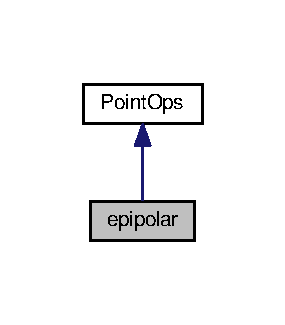
\includegraphics[width=137pt]{classepipolar__inherit__graph}
\end{center}
\end{figure}


Collaboration diagram for epipolar\+:\nopagebreak
\begin{figure}[H]
\begin{center}
\leavevmode
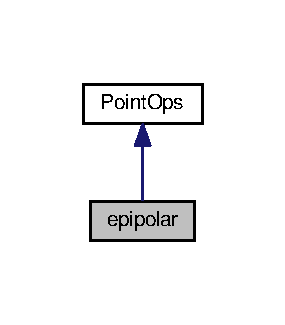
\includegraphics[width=137pt]{classepipolar__coll__graph}
\end{center}
\end{figure}
\subsection*{Public Member Functions}
\begin{DoxyCompactItemize}
\item 
\hyperlink{classepipolar_af5946f7532025b261a04dac12e18946d}{epipolar} ()
\begin{DoxyCompactList}\small\item\em Constructor for the epipolar class. \end{DoxyCompactList}\item 
Eigen\+::\+Matrix3d \hyperlink{classepipolar_a704a496c08556dac8133ec1b403e728c}{get\+Camera\+Params} (char filename\+\_\+calib\mbox{[}200\mbox{]})
\begin{DoxyCompactList}\small\item\em Gets camera parameters from the calib.\+txt files in the dataset. The folder structure is assumed to be similar to the K\+I\+T\+TI dataset. \end{DoxyCompactList}\item 
double \hyperlink{classepipolar_a7afbdbd2643ef41ca10bd7ad053f3762}{get\+Absolute\+Scale} (char filename\+\_\+gt\mbox{[}200\mbox{]}, int frame\+\_\+id)
\begin{DoxyCompactList}\small\item\em Gets scale from ground truth file depending on the image sequence, from the pose folder. \end{DoxyCompactList}\item 
void \hyperlink{classepipolar_a7c50ca7a4431c5e08a848bed9dba878e}{estimate\+Fundamental\+Matrix} (Eigen\+::\+Matrix\+Xd \&points1, Eigen\+::\+Matrix\+Xd \&points2, Eigen\+::\+Matrix3d \&F)
\begin{DoxyCompactList}\small\item\em Estimates fundamental matrix from matched points. Takes in the matrix F by reference which is updated. \end{DoxyCompactList}\item 
void \hyperlink{classepipolar_a8530a3ec65e1915ee7df1c555c74014e}{Fundamental\+Mat\+R\+A\+N\+S\+AC} (Eigen\+::\+Matrix3d \&F, Eigen\+::\+Matrix\+Xd \&points1, Eigen\+::\+Matrix\+Xd \&points2)
\begin{DoxyCompactList}\small\item\em Uses R\+A\+N\+S\+AC to refine the Fundamental matrix. This takes advantage of the fact that the features lie on the epipolar plane. \end{DoxyCompactList}\item 
Eigen\+::\+Matrix\+Xd \hyperlink{classepipolar_ad5ce6ee9ac5df7f8f02e4c48686cc637}{compute\+Epipole} (Eigen\+::\+Matrix3d \&F)
\begin{DoxyCompactList}\small\item\em Computes epipole based on the idea that the epipoles lie on the epipolar plane. So Linear Least Squares to solve e2\+T$\ast$\+F$\ast$e1 = 0. \end{DoxyCompactList}\end{DoxyCompactItemize}


\subsection{Detailed Description}
Definition of the epipolar class. It contains all the functions and variables required to compute epipolar geometry. 

The sole purpose of this class is to compute geometry based on matched points. Inherits the \hyperlink{class_point_ops}{Point\+Ops} class and uses the mathematical conversion methods from it. 

\subsection{Constructor \& Destructor Documentation}
\index{epipolar@{epipolar}!epipolar@{epipolar}}
\index{epipolar@{epipolar}!epipolar@{epipolar}}
\subsubsection[{\texorpdfstring{epipolar()}{epipolar()}}]{\setlength{\rightskip}{0pt plus 5cm}epipolar\+::epipolar (
\begin{DoxyParamCaption}
{}
\end{DoxyParamCaption}
)}\hypertarget{classepipolar_af5946f7532025b261a04dac12e18946d}{}\label{classepipolar_af5946f7532025b261a04dac12e18946d}


Constructor for the epipolar class. 

Initializes the camera matrix to default values in the event of file reading failure. Initializes R\+A\+N\+S\+AC variables. 

\subsection{Member Function Documentation}
\index{epipolar@{epipolar}!compute\+Epipole@{compute\+Epipole}}
\index{compute\+Epipole@{compute\+Epipole}!epipolar@{epipolar}}
\subsubsection[{\texorpdfstring{compute\+Epipole(\+Eigen\+::\+Matrix3d \&\+F)}{computeEpipole(Eigen::Matrix3d &F)}}]{\setlength{\rightskip}{0pt plus 5cm}Eigen\+::\+Matrix\+Xd epipolar\+::compute\+Epipole (
\begin{DoxyParamCaption}
\item[{Eigen\+::\+Matrix3d \&}]{F}
\end{DoxyParamCaption}
)}\hypertarget{classepipolar_ad5ce6ee9ac5df7f8f02e4c48686cc637}{}\label{classepipolar_ad5ce6ee9ac5df7f8f02e4c48686cc637}


Computes epipole based on the idea that the epipoles lie on the epipolar plane. So Linear Least Squares to solve e2\+T$\ast$\+F$\ast$e1 = 0. 

Takes in the Fundamental matrix and returns a 3x2 matrix in homogenous form, with the coordinates for the epipole. \index{epipolar@{epipolar}!estimate\+Fundamental\+Matrix@{estimate\+Fundamental\+Matrix}}
\index{estimate\+Fundamental\+Matrix@{estimate\+Fundamental\+Matrix}!epipolar@{epipolar}}
\subsubsection[{\texorpdfstring{estimate\+Fundamental\+Matrix(\+Eigen\+::\+Matrix\+Xd \&points1, Eigen\+::\+Matrix\+Xd \&points2, Eigen\+::\+Matrix3d \&\+F)}{estimateFundamentalMatrix(Eigen::MatrixXd &points1, Eigen::MatrixXd &points2, Eigen::Matrix3d &F)}}]{\setlength{\rightskip}{0pt plus 5cm}void epipolar\+::estimate\+Fundamental\+Matrix (
\begin{DoxyParamCaption}
\item[{Eigen\+::\+Matrix\+Xd \&}]{points1, }
\item[{Eigen\+::\+Matrix\+Xd \&}]{points2, }
\item[{Eigen\+::\+Matrix3d \&}]{F}
\end{DoxyParamCaption}
)}\hypertarget{classepipolar_a7c50ca7a4431c5e08a848bed9dba878e}{}\label{classepipolar_a7c50ca7a4431c5e08a848bed9dba878e}


Estimates fundamental matrix from matched points. Takes in the matrix F by reference which is updated. 

This version uses the 8 point algorithm and solves the Linear Least Squares problem Ax = 0 using S\+VD. The method can take more than 8 points and still compute the matrix. Takes in the matched points in the form of a 3xN matrix of homogenous coordinates. 

Here is the call graph for this function\+:\nopagebreak
\begin{figure}[H]
\begin{center}
\leavevmode
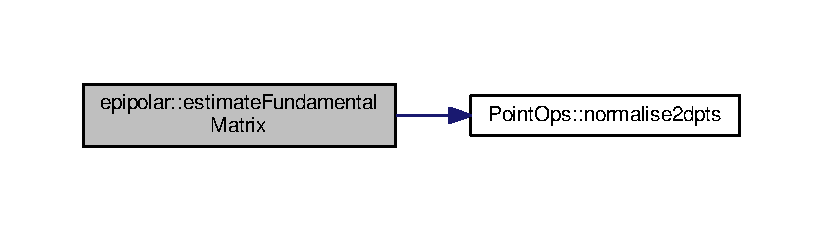
\includegraphics[width=350pt]{classepipolar_a7c50ca7a4431c5e08a848bed9dba878e_cgraph}
\end{center}
\end{figure}


\index{epipolar@{epipolar}!Fundamental\+Mat\+R\+A\+N\+S\+AC@{Fundamental\+Mat\+R\+A\+N\+S\+AC}}
\index{Fundamental\+Mat\+R\+A\+N\+S\+AC@{Fundamental\+Mat\+R\+A\+N\+S\+AC}!epipolar@{epipolar}}
\subsubsection[{\texorpdfstring{Fundamental\+Mat\+R\+A\+N\+S\+A\+C(\+Eigen\+::\+Matrix3d \&\+F, Eigen\+::\+Matrix\+Xd \&points1, Eigen\+::\+Matrix\+Xd \&points2)}{FundamentalMatRANSAC(Eigen::Matrix3d &F, Eigen::MatrixXd &points1, Eigen::MatrixXd &points2)}}]{\setlength{\rightskip}{0pt plus 5cm}void epipolar\+::\+Fundamental\+Mat\+R\+A\+N\+S\+AC (
\begin{DoxyParamCaption}
\item[{Eigen\+::\+Matrix3d \&}]{F, }
\item[{Eigen\+::\+Matrix\+Xd \&}]{points1, }
\item[{Eigen\+::\+Matrix\+Xd \&}]{points2}
\end{DoxyParamCaption}
)}\hypertarget{classepipolar_a8530a3ec65e1915ee7df1c555c74014e}{}\label{classepipolar_a8530a3ec65e1915ee7df1c555c74014e}


Uses R\+A\+N\+S\+AC to refine the Fundamental matrix. This takes advantage of the fact that the features lie on the epipolar plane. 

Uses x2\+T$\ast$\+F$\ast$x1 = 0 as a distance function for the R\+A\+N\+S\+AC. Once inliers are selected, a final fundamental matrix is computed using them. 

Here is the call graph for this function\+:
\nopagebreak
\begin{figure}[H]
\begin{center}
\leavevmode
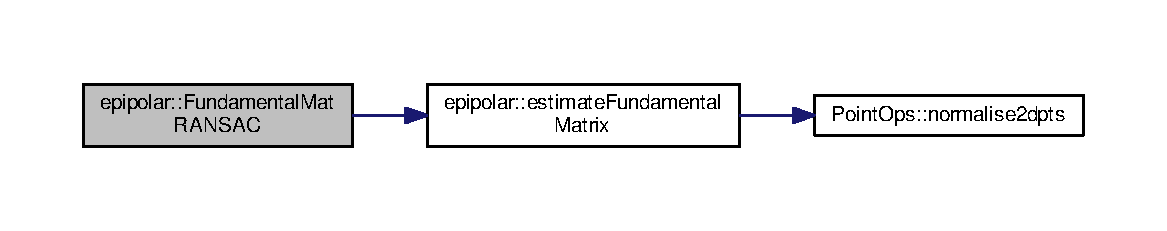
\includegraphics[width=350pt]{classepipolar_a8530a3ec65e1915ee7df1c555c74014e_cgraph}
\end{center}
\end{figure}


\index{epipolar@{epipolar}!get\+Absolute\+Scale@{get\+Absolute\+Scale}}
\index{get\+Absolute\+Scale@{get\+Absolute\+Scale}!epipolar@{epipolar}}
\subsubsection[{\texorpdfstring{get\+Absolute\+Scale(char filename\+\_\+gt[200], int frame\+\_\+id)}{getAbsoluteScale(char filename_gt[200], int frame_id)}}]{\setlength{\rightskip}{0pt plus 5cm}double epipolar\+::get\+Absolute\+Scale (
\begin{DoxyParamCaption}
\item[{char}]{filename\+\_\+gt\mbox{[}200\mbox{]}, }
\item[{int}]{frame\+\_\+id}
\end{DoxyParamCaption}
)}\hypertarget{classepipolar_a7afbdbd2643ef41ca10bd7ad053f3762}{}\label{classepipolar_a7afbdbd2643ef41ca10bd7ad053f3762}


Gets scale from ground truth file depending on the image sequence, from the pose folder. 

Ground truth is used to get scale for this application. This can be switched out to get scale from another source, like a speedometer. \index{epipolar@{epipolar}!get\+Camera\+Params@{get\+Camera\+Params}}
\index{get\+Camera\+Params@{get\+Camera\+Params}!epipolar@{epipolar}}
\subsubsection[{\texorpdfstring{get\+Camera\+Params(char filename\+\_\+calib[200])}{getCameraParams(char filename_calib[200])}}]{\setlength{\rightskip}{0pt plus 5cm}Eigen\+::\+Matrix3d epipolar\+::get\+Camera\+Params (
\begin{DoxyParamCaption}
\item[{char}]{filename\+\_\+calib\mbox{[}200\mbox{]}}
\end{DoxyParamCaption}
)}\hypertarget{classepipolar_a704a496c08556dac8133ec1b403e728c}{}\label{classepipolar_a704a496c08556dac8133ec1b403e728c}


Gets camera parameters from the calib.\+txt files in the dataset. The folder structure is assumed to be similar to the K\+I\+T\+TI dataset. 

Reads the parameters from the text files and stores it in the K matrix parameter. If reading the file fails, default values are used. 

The documentation for this class was generated from the following files\+:\begin{DoxyCompactItemize}
\item 
/home/yashmanian/\+C\+P\+P/\+Monocular\+V\+O/include/\hyperlink{epipolar_8hpp}{epipolar.\+hpp}\item 
/home/yashmanian/\+C\+P\+P/\+Monocular\+V\+O/src/src\+Files/\hyperlink{epipolar_8cpp}{epipolar.\+cpp}\end{DoxyCompactItemize}

\hypertarget{class_feat_track}{}\section{Feat\+Track Class Reference}
\label{class_feat_track}\index{Feat\+Track@{Feat\+Track}}


Definition of the \hyperlink{class_feat_track}{Feat\+Track} class. It contains all the functions and variables for detection, tracking and computing homography.  




{\ttfamily \#include $<$Feat\+Track.\+hpp$>$}

\subsection*{Public Member Functions}
\begin{DoxyCompactItemize}
\item 
\hyperlink{class_feat_track_a1155bdc5bde9a95519354144f9920beb}{Feat\+Track} ()
\begin{DoxyCompactList}\small\item\em Constructor for the \hyperlink{class_feat_track}{Feat\+Track} class. \end{DoxyCompactList}\item 
void \hyperlink{class_feat_track_ab1dd27505ee431ded0b68a32d959410b}{feature\+Tracking} (cv\+::\+Mat img\+\_\+1, cv\+::\+Mat img\+\_\+2, std\+::vector$<$ cv\+::\+Point2f $>$ \&img\+\_\+1\+\_\+points, std\+::vector$<$ cv\+::\+Point2f $>$ \&img\+\_\+2\+\_\+points, std\+::vector$<$ uchar $>$ \&status)
\begin{DoxyCompactList}\small\item\em Calculates flow between two images based on detected features. \end{DoxyCompactList}\item 
void \hyperlink{class_feat_track_ae0c07b941c44dd1bf32d866611561835}{feature\+Detection} (cv\+::\+Mat img\+\_\+1, std\+::vector$<$ cv\+::\+Point2f $>$ \&img\+\_\+points)
\begin{DoxyCompactList}\small\item\em Detects F\+A\+ST features on the input image. \end{DoxyCompactList}\item 
void \hyperlink{class_feat_track_a46b14a758dd70d9a6e7a70f0cdfaa347}{compute\+Homography} (std\+::vector$<$ cv\+::\+Point2f $>$ \&x1, std\+::vector$<$ cv\+::\+Point2f $>$ \&x2, cv\+::\+Mat \&H)
\begin{DoxyCompactList}\small\item\em Computes homography between two images. \end{DoxyCompactList}\item 
void \hyperlink{class_feat_track_abb6e503ee7c4eaed6c00d386d797f35a}{homography\+R\+A\+N\+S\+AC} (std\+::vector$<$ cv\+::\+Point2f $>$ \&img\+\_\+1\+\_\+points, std\+::vector$<$ cv\+::\+Point2f $>$ \&img\+\_\+2\+\_\+points)
\begin{DoxyCompactList}\small\item\em Uses R\+A\+N\+S\+AC to refine the Homography matrix. \end{DoxyCompactList}\end{DoxyCompactItemize}


\subsection{Detailed Description}
Definition of the \hyperlink{class_feat_track}{Feat\+Track} class. It contains all the functions and variables for detection, tracking and computing homography. 

\subsection{Constructor \& Destructor Documentation}
\index{Feat\+Track@{Feat\+Track}!Feat\+Track@{Feat\+Track}}
\index{Feat\+Track@{Feat\+Track}!Feat\+Track@{Feat\+Track}}
\subsubsection[{\texorpdfstring{Feat\+Track()}{FeatTrack()}}]{\setlength{\rightskip}{0pt plus 5cm}Feat\+Track\+::\+Feat\+Track (
\begin{DoxyParamCaption}
{}
\end{DoxyParamCaption}
)}\hypertarget{class_feat_track_a1155bdc5bde9a95519354144f9920beb}{}\label{class_feat_track_a1155bdc5bde9a95519354144f9920beb}


Constructor for the \hyperlink{class_feat_track}{Feat\+Track} class. 

Initializes the flow calculation parameters and homography R\+A\+N\+S\+AC parameters. 

\subsection{Member Function Documentation}
\index{Feat\+Track@{Feat\+Track}!compute\+Homography@{compute\+Homography}}
\index{compute\+Homography@{compute\+Homography}!Feat\+Track@{Feat\+Track}}
\subsubsection[{\texorpdfstring{compute\+Homography(std\+::vector$<$ cv\+::\+Point2f $>$ \&x1, std\+::vector$<$ cv\+::\+Point2f $>$ \&x2, cv\+::\+Mat \&\+H)}{computeHomography(std::vector< cv::Point2f > &x1, std::vector< cv::Point2f > &x2, cv::Mat &H)}}]{\setlength{\rightskip}{0pt plus 5cm}void Feat\+Track\+::compute\+Homography (
\begin{DoxyParamCaption}
\item[{std\+::vector$<$ cv\+::\+Point2f $>$ \&}]{x1, }
\item[{std\+::vector$<$ cv\+::\+Point2f $>$ \&}]{x2, }
\item[{cv\+::\+Mat \&}]{H}
\end{DoxyParamCaption}
)}\hypertarget{class_feat_track_a46b14a758dd70d9a6e7a70f0cdfaa347}{}\label{class_feat_track_a46b14a758dd70d9a6e7a70f0cdfaa347}


Computes homography between two images. 

Takes in four matched points from each image to compute affine transform. \index{Feat\+Track@{Feat\+Track}!feature\+Detection@{feature\+Detection}}
\index{feature\+Detection@{feature\+Detection}!Feat\+Track@{Feat\+Track}}
\subsubsection[{\texorpdfstring{feature\+Detection(cv\+::\+Mat img\+\_\+1, std\+::vector$<$ cv\+::\+Point2f $>$ \&img\+\_\+points)}{featureDetection(cv::Mat img_1, std::vector< cv::Point2f > &img_points)}}]{\setlength{\rightskip}{0pt plus 5cm}void Feat\+Track\+::feature\+Detection (
\begin{DoxyParamCaption}
\item[{cv\+::\+Mat}]{img\+\_\+1, }
\item[{std\+::vector$<$ cv\+::\+Point2f $>$ \&}]{img\+\_\+points}
\end{DoxyParamCaption}
)}\hypertarget{class_feat_track_ae0c07b941c44dd1bf32d866611561835}{}\label{class_feat_track_ae0c07b941c44dd1bf32d866611561835}


Detects F\+A\+ST features on the input image. 

Takes in image and an empty vector to store points. \index{Feat\+Track@{Feat\+Track}!feature\+Tracking@{feature\+Tracking}}
\index{feature\+Tracking@{feature\+Tracking}!Feat\+Track@{Feat\+Track}}
\subsubsection[{\texorpdfstring{feature\+Tracking(cv\+::\+Mat img\+\_\+1, cv\+::\+Mat img\+\_\+2, std\+::vector$<$ cv\+::\+Point2f $>$ \&img\+\_\+1\+\_\+points, std\+::vector$<$ cv\+::\+Point2f $>$ \&img\+\_\+2\+\_\+points, std\+::vector$<$ uchar $>$ \&status)}{featureTracking(cv::Mat img_1, cv::Mat img_2, std::vector< cv::Point2f > &img_1_points, std::vector< cv::Point2f > &img_2_points, std::vector< uchar > &status)}}]{\setlength{\rightskip}{0pt plus 5cm}void Feat\+Track\+::feature\+Tracking (
\begin{DoxyParamCaption}
\item[{cv\+::\+Mat}]{img\+\_\+1, }
\item[{cv\+::\+Mat}]{img\+\_\+2, }
\item[{std\+::vector$<$ cv\+::\+Point2f $>$ \&}]{img\+\_\+1\+\_\+points, }
\item[{std\+::vector$<$ cv\+::\+Point2f $>$ \&}]{img\+\_\+2\+\_\+points, }
\item[{std\+::vector$<$ uchar $>$ \&}]{status}
\end{DoxyParamCaption}
)}\hypertarget{class_feat_track_ab1dd27505ee431ded0b68a32d959410b}{}\label{class_feat_track_ab1dd27505ee431ded0b68a32d959410b}


Calculates flow between two images based on detected features. 

Takes in the two images in the cv\+::\+Mat format, and a vector of features from the first image, and a vector of characters to emphasize match. \index{Feat\+Track@{Feat\+Track}!homography\+R\+A\+N\+S\+AC@{homography\+R\+A\+N\+S\+AC}}
\index{homography\+R\+A\+N\+S\+AC@{homography\+R\+A\+N\+S\+AC}!Feat\+Track@{Feat\+Track}}
\subsubsection[{\texorpdfstring{homography\+R\+A\+N\+S\+A\+C(std\+::vector$<$ cv\+::\+Point2f $>$ \&img\+\_\+1\+\_\+points, std\+::vector$<$ cv\+::\+Point2f $>$ \&img\+\_\+2\+\_\+points)}{homographyRANSAC(std::vector< cv::Point2f > &img_1_points, std::vector< cv::Point2f > &img_2_points)}}]{\setlength{\rightskip}{0pt plus 5cm}void Feat\+Track\+::homography\+R\+A\+N\+S\+AC (
\begin{DoxyParamCaption}
\item[{std\+::vector$<$ cv\+::\+Point2f $>$ \&}]{img\+\_\+1\+\_\+points, }
\item[{std\+::vector$<$ cv\+::\+Point2f $>$ \&}]{img\+\_\+2\+\_\+points}
\end{DoxyParamCaption}
)}\hypertarget{class_feat_track_abb6e503ee7c4eaed6c00d386d797f35a}{}\label{class_feat_track_abb6e503ee7c4eaed6c00d386d797f35a}


Uses R\+A\+N\+S\+AC to refine the Homography matrix. 

Uses compute\+Homography as a distance function for the R\+A\+N\+S\+AC. Once inliers are selected, a final Homography matrix is computed using them. 

Here is the call graph for this function\+:\nopagebreak
\begin{figure}[H]
\begin{center}
\leavevmode
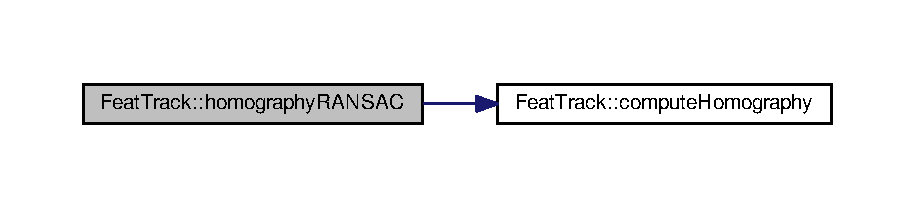
\includegraphics[width=350pt]{class_feat_track_abb6e503ee7c4eaed6c00d386d797f35a_cgraph}
\end{center}
\end{figure}




The documentation for this class was generated from the following files\+:\begin{DoxyCompactItemize}
\item 
/home/yashmanian/\+C\+P\+P/\+Monocular\+V\+O/include/\hyperlink{_feat_track_8hpp}{Feat\+Track.\+hpp}\item 
/home/yashmanian/\+C\+P\+P/\+Monocular\+V\+O/src/src\+Files/\hyperlink{_feat_track_8cpp}{Feat\+Track.\+cpp}\end{DoxyCompactItemize}

\hypertarget{class_point_ops}{}\section{Point\+Ops Class Reference}
\label{class_point_ops}\index{Point\+Ops@{Point\+Ops}}


Definition of the \hyperlink{class_point_ops}{Point\+Ops} class. It contains all the functions and variables required manipulate point formats.  




{\ttfamily \#include $<$Point\+Ops.\+hpp$>$}



Inheritance diagram for Point\+Ops\+:\nopagebreak
\begin{figure}[H]
\begin{center}
\leavevmode
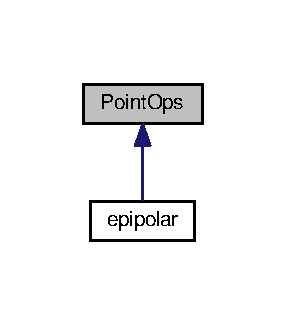
\includegraphics[width=137pt]{class_point_ops__inherit__graph}
\end{center}
\end{figure}
\subsection*{Public Member Functions}
\begin{DoxyCompactItemize}
\item 
Eigen\+::\+Matrix\+Xd \hyperlink{class_point_ops_aedd3f88c0e3eccd17085585cdd85319a}{normalise2dpts} (Eigen\+::\+Matrix\+Xd \&pts)
\begin{DoxyCompactList}\small\item\em Normalises the point set around its centroid. \end{DoxyCompactList}\item 
Eigen\+::\+Matrix\+Xd \hyperlink{class_point_ops_a850c1cf8569537a6ec70dc2721c4ab1f}{cv2\+Eigen\+Homogenous} (std\+::vector$<$ cv\+::\+Point2f $>$ \&pts)
\begin{DoxyCompactList}\small\item\em Converts a vector of 2D points to a 3xN matrix of homogenous points. \end{DoxyCompactList}\end{DoxyCompactItemize}


\subsection{Detailed Description}
Definition of the \hyperlink{class_point_ops}{Point\+Ops} class. It contains all the functions and variables required manipulate point formats. 

This class will contain methods to run mathematical operations on sets of matched points. 

\subsection{Member Function Documentation}
\index{Point\+Ops@{Point\+Ops}!cv2\+Eigen\+Homogenous@{cv2\+Eigen\+Homogenous}}
\index{cv2\+Eigen\+Homogenous@{cv2\+Eigen\+Homogenous}!Point\+Ops@{Point\+Ops}}
\subsubsection[{\texorpdfstring{cv2\+Eigen\+Homogenous(std\+::vector$<$ cv\+::\+Point2f $>$ \&pts)}{cv2EigenHomogenous(std::vector< cv::Point2f > &pts)}}]{\setlength{\rightskip}{0pt plus 5cm}Eigen\+::\+Matrix\+Xd Point\+Ops\+::cv2\+Eigen\+Homogenous (
\begin{DoxyParamCaption}
\item[{std\+::vector$<$ cv\+::\+Point2f $>$ \&}]{pts}
\end{DoxyParamCaption}
)}\hypertarget{class_point_ops_a850c1cf8569537a6ec70dc2721c4ab1f}{}\label{class_point_ops_a850c1cf8569537a6ec70dc2721c4ab1f}


Converts a vector of 2D points to a 3xN matrix of homogenous points. 

Allows conversion from open\+CV Point2f features to Eigen Matrices. \index{Point\+Ops@{Point\+Ops}!normalise2dpts@{normalise2dpts}}
\index{normalise2dpts@{normalise2dpts}!Point\+Ops@{Point\+Ops}}
\subsubsection[{\texorpdfstring{normalise2dpts(\+Eigen\+::\+Matrix\+Xd \&pts)}{normalise2dpts(Eigen::MatrixXd &pts)}}]{\setlength{\rightskip}{0pt plus 5cm}Eigen\+::\+Matrix\+Xd Point\+Ops\+::normalise2dpts (
\begin{DoxyParamCaption}
\item[{Eigen\+::\+Matrix\+Xd \&}]{pts}
\end{DoxyParamCaption}
)}\hypertarget{class_point_ops_aedd3f88c0e3eccd17085585cdd85319a}{}\label{class_point_ops_aedd3f88c0e3eccd17085585cdd85319a}


Normalises the point set around its centroid. 

Takes in a 3xN matrix of points and returns a 3xN matrix of normalised homogenous coordinates. 

The documentation for this class was generated from the following files\+:\begin{DoxyCompactItemize}
\item 
/home/yashmanian/\+C\+P\+P/\+Monocular\+V\+O/include/\hyperlink{_point_ops_8hpp}{Point\+Ops.\+hpp}\item 
/home/yashmanian/\+C\+P\+P/\+Monocular\+V\+O/src/src\+Files/\hyperlink{_point_ops_8cpp}{Point\+Ops.\+cpp}\end{DoxyCompactItemize}

\chapter{File Documentation}
\hypertarget{epipolar_8hpp}{}\section{/home/yashmanian/\+C\+P\+P/\+Monocular\+V\+O/include/epipolar.hpp File Reference}
\label{epipolar_8hpp}\index{/home/yashmanian/\+C\+P\+P/\+Monocular\+V\+O/include/epipolar.\+hpp@{/home/yashmanian/\+C\+P\+P/\+Monocular\+V\+O/include/epipolar.\+hpp}}


Header file with definitions for class epipolar.  


{\ttfamily \#include \char`\"{}opencv2/video/tracking.\+hpp\char`\"{}}\\*
{\ttfamily \#include \char`\"{}opencv2/imgproc/imgproc.\+hpp\char`\"{}}\\*
{\ttfamily \#include \char`\"{}opencv2/highgui/highgui.\+hpp\char`\"{}}\\*
{\ttfamily \#include \char`\"{}opencv2/features2d/features2d.\+hpp\char`\"{}}\\*
{\ttfamily \#include \char`\"{}opencv2/calib3d/calib3d.\+hpp\char`\"{}}\\*
{\ttfamily \#include $<$iostream$>$}\\*
{\ttfamily \#include $<$ctype.\+h$>$}\\*
{\ttfamily \#include $<$vector$>$}\\*
{\ttfamily \#include $<$ctime$>$}\\*
{\ttfamily \#include $<$sstream$>$}\\*
{\ttfamily \#include $<$fstream$>$}\\*
{\ttfamily \#include $<$string$>$}\\*
{\ttfamily \#include $<$Eigen/\+Dense$>$}\\*
{\ttfamily \#include $<$Eigen/\+S\+VD$>$}\\*
{\ttfamily \#include $<$Eigen/\+Core$>$}\\*
{\ttfamily \#include \char`\"{}Point\+Ops.\+hpp\char`\"{}}\\*
Include dependency graph for epipolar.\+hpp\+:\nopagebreak
\begin{figure}[H]
\begin{center}
\leavevmode
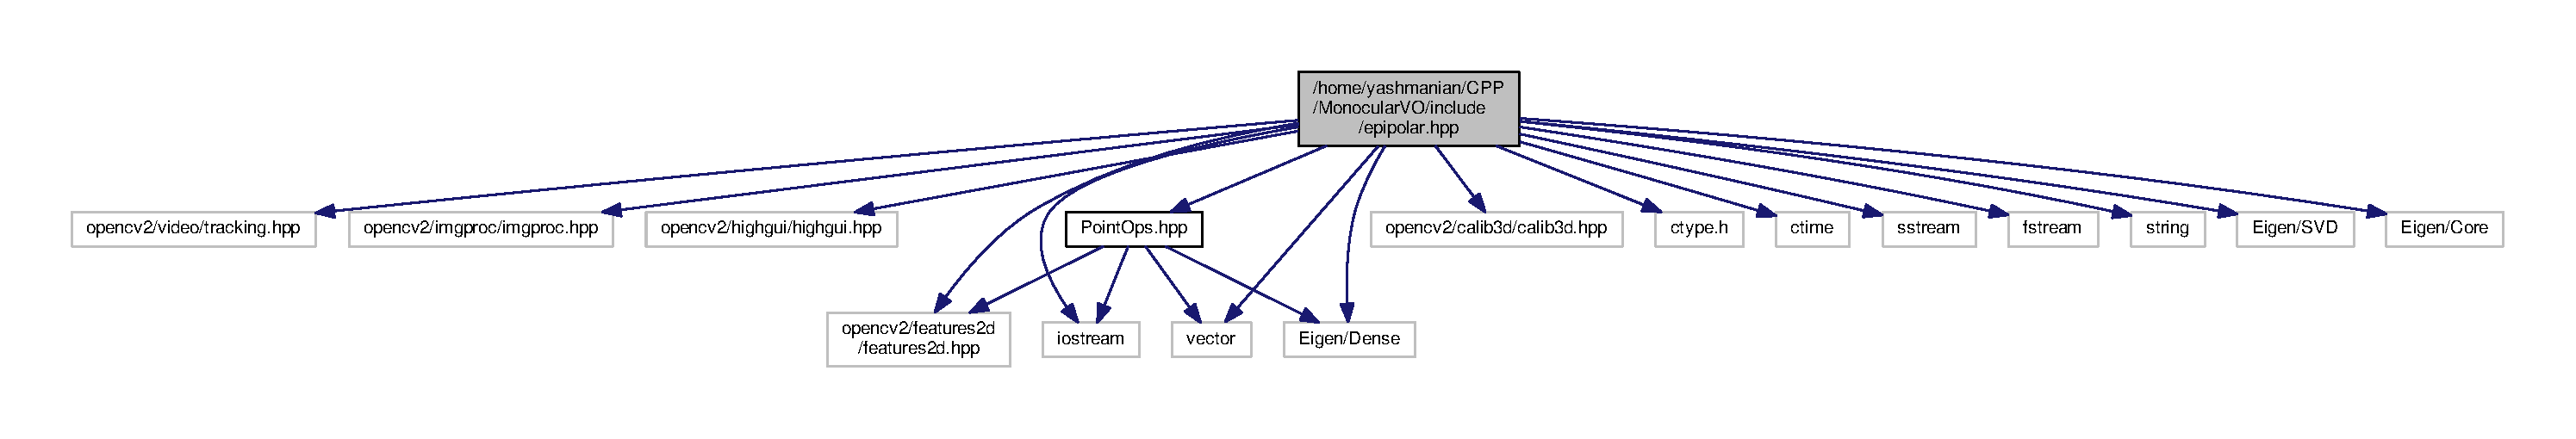
\includegraphics[width=350pt]{epipolar_8hpp__incl}
\end{center}
\end{figure}
This graph shows which files directly or indirectly include this file\+:\nopagebreak
\begin{figure}[H]
\begin{center}
\leavevmode
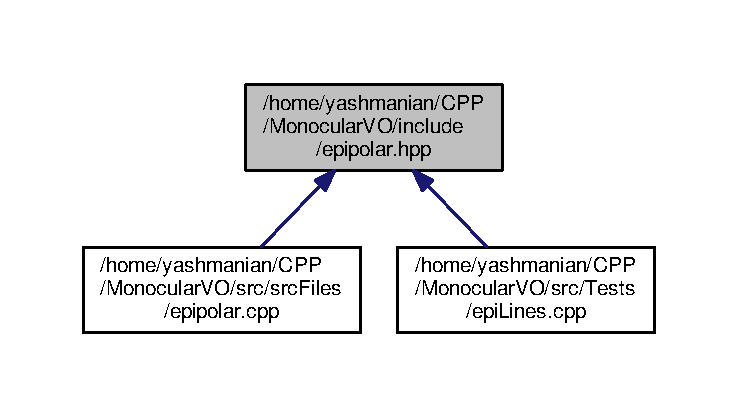
\includegraphics[width=350pt]{epipolar_8hpp__dep__incl}
\end{center}
\end{figure}
\subsection*{Classes}
\begin{DoxyCompactItemize}
\item 
class \hyperlink{classepipolar}{epipolar}
\begin{DoxyCompactList}\small\item\em Definition of the epipolar class. It contains all the functions and variables required to compute epipolar geometry. \end{DoxyCompactList}\end{DoxyCompactItemize}


\subsection{Detailed Description}
Header file with definitions for class epipolar. 

M\+IT License Copyright (c) 2018 Yash Manian Permission is hereby granted, free of charge, to any person obtaining a copy of this software and associated documentation files (the \char`\"{}\+Software\char`\"{}), to deal in the Software without restriction, including without limitation the rights to use, copy, modify, merge, publish, distribute, sublicense, and/or sell copies of the Software, and to permit persons to whom the Software is furnished to do so, subject to the following conditions\+: The above copyright notice and this permission notice shall be included in all copies or substantial portions of the Software. T\+HE S\+O\+F\+T\+W\+A\+RE IS P\+R\+O\+V\+I\+D\+ED \char`\"{}\+A\+S I\+S\char`\"{}, W\+I\+T\+H\+O\+UT W\+A\+R\+R\+A\+N\+TY OF A\+NY K\+I\+ND, E\+X\+P\+R\+E\+SS OR I\+M\+P\+L\+I\+ED, I\+N\+C\+L\+U\+D\+I\+NG B\+UT N\+OT L\+I\+M\+I\+T\+ED TO T\+HE W\+A\+R\+R\+A\+N\+T\+I\+ES OF M\+E\+R\+C\+H\+A\+N\+T\+A\+B\+I\+L\+I\+TY, F\+I\+T\+N\+E\+SS F\+OR A P\+A\+R\+T\+I\+C\+U\+L\+AR P\+U\+R\+P\+O\+SE A\+ND N\+O\+N\+I\+N\+F\+R\+I\+N\+G\+E\+M\+E\+NT. IN NO E\+V\+E\+NT S\+H\+A\+LL T\+HE A\+U\+T\+H\+O\+RS OR C\+O\+P\+Y\+R\+I\+G\+HT H\+O\+L\+D\+E\+RS BE L\+I\+A\+B\+LE F\+OR A\+NY C\+L\+A\+IM, D\+A\+M\+A\+G\+ES OR O\+T\+H\+ER L\+I\+A\+B\+I\+L\+I\+TY, W\+H\+E\+T\+H\+ER IN AN A\+C\+T\+I\+ON OF C\+O\+N\+T\+R\+A\+CT, T\+O\+RT OR O\+T\+H\+E\+R\+W\+I\+SE, A\+R\+I\+S\+I\+NG F\+R\+OM, O\+UT OF OR IN C\+O\+N\+N\+E\+C\+T\+I\+ON W\+I\+TH T\+HE S\+O\+F\+T\+W\+A\+RE OR T\+HE U\+SE OR O\+T\+H\+ER D\+E\+A\+L\+I\+N\+GS IN T\+HE S\+O\+F\+T\+W\+A\+RE.

\begin{DoxyCopyright}{Copyright}
Copyright 2018 Yash Manian
\end{DoxyCopyright}
\begin{DoxyAuthor}{Author}
Yash Manian Declaration of methods to compute Epipolar constraints 
\end{DoxyAuthor}

\hypertarget{_feat_track_8hpp}{}\section{/home/yashmanian/\+C\+P\+P/\+Monocular\+V\+O/include/\+Feat\+Track.hpp File Reference}
\label{_feat_track_8hpp}\index{/home/yashmanian/\+C\+P\+P/\+Monocular\+V\+O/include/\+Feat\+Track.\+hpp@{/home/yashmanian/\+C\+P\+P/\+Monocular\+V\+O/include/\+Feat\+Track.\+hpp}}


Header file with definitions for class \hyperlink{class_feat_track}{Feat\+Track}.  


{\ttfamily \#include \char`\"{}opencv2/video/tracking.\+hpp\char`\"{}}\\*
{\ttfamily \#include \char`\"{}opencv2/imgproc/imgproc.\+hpp\char`\"{}}\\*
{\ttfamily \#include \char`\"{}opencv2/highgui/highgui.\+hpp\char`\"{}}\\*
{\ttfamily \#include \char`\"{}opencv2/features2d/features2d.\+hpp\char`\"{}}\\*
{\ttfamily \#include \char`\"{}opencv2/calib3d/calib3d.\+hpp\char`\"{}}\\*
{\ttfamily \#include $<$iostream$>$}\\*
{\ttfamily \#include $<$ctype.\+h$>$}\\*
{\ttfamily \#include $<$math.\+h$>$}\\*
{\ttfamily \#include $<$vector$>$}\\*
{\ttfamily \#include $<$ctime$>$}\\*
{\ttfamily \#include $<$sstream$>$}\\*
{\ttfamily \#include $<$fstream$>$}\\*
{\ttfamily \#include $<$string$>$}\\*
Include dependency graph for Feat\+Track.\+hpp\+:\nopagebreak
\begin{figure}[H]
\begin{center}
\leavevmode
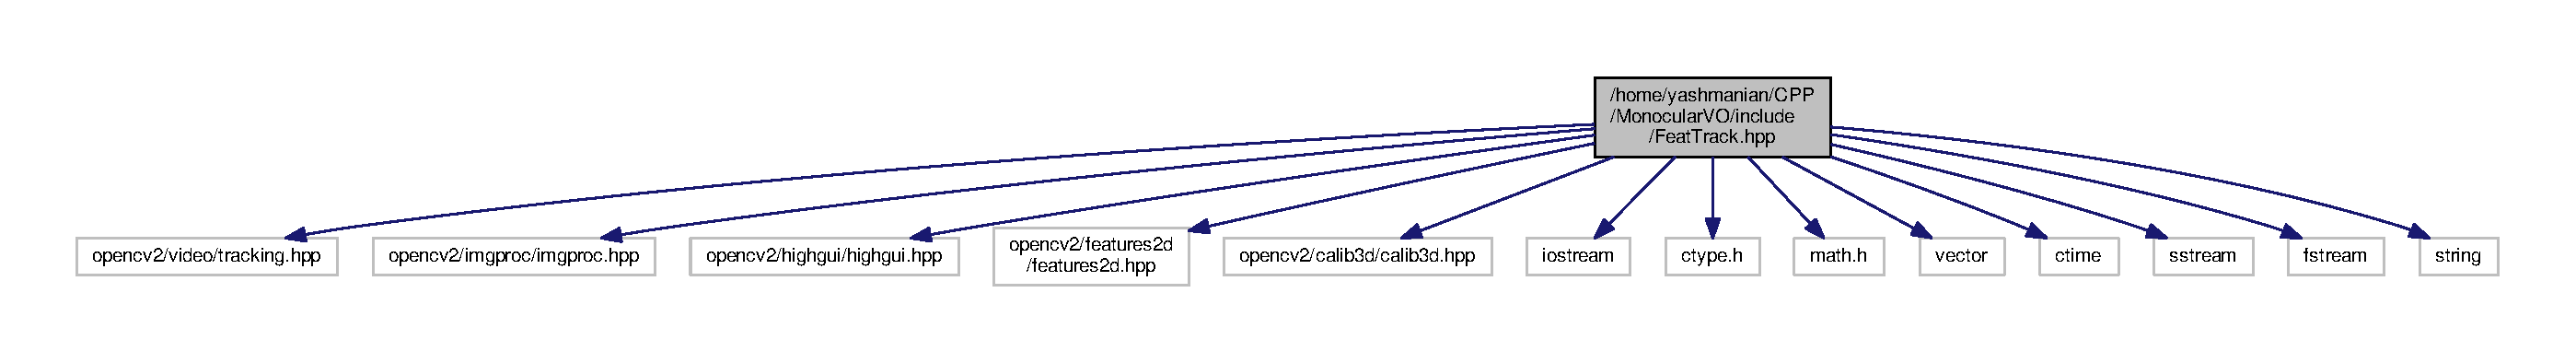
\includegraphics[width=350pt]{_feat_track_8hpp__incl}
\end{center}
\end{figure}
This graph shows which files directly or indirectly include this file\+:\nopagebreak
\begin{figure}[H]
\begin{center}
\leavevmode
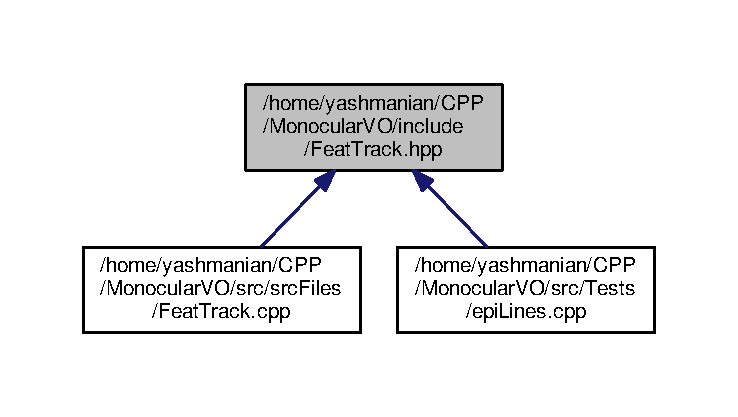
\includegraphics[width=350pt]{_feat_track_8hpp__dep__incl}
\end{center}
\end{figure}
\subsection*{Classes}
\begin{DoxyCompactItemize}
\item 
class \hyperlink{class_feat_track}{Feat\+Track}
\begin{DoxyCompactList}\small\item\em Definition of the \hyperlink{class_feat_track}{Feat\+Track} class. It contains all the functions and variables for detection, tracking and computing homography. \end{DoxyCompactList}\end{DoxyCompactItemize}


\subsection{Detailed Description}
Header file with definitions for class \hyperlink{class_feat_track}{Feat\+Track}. 

M\+IT License Copyright (c) 2018 Yash Manian Permission is hereby granted, free of charge, to any person obtaining a copy of this software and associated documentation files (the \char`\"{}\+Software\char`\"{}), to deal in the Software without restriction, including without limitation the rights to use, copy, modify, merge, publish, distribute, sublicense, and/or sell copies of the Software, and to permit persons to whom the Software is furnished to do so, subject to the following conditions\+: The above copyright notice and this permission notice shall be included in all copies or substantial portions of the Software. T\+HE S\+O\+F\+T\+W\+A\+RE IS P\+R\+O\+V\+I\+D\+ED \char`\"{}\+A\+S I\+S\char`\"{}, W\+I\+T\+H\+O\+UT W\+A\+R\+R\+A\+N\+TY OF A\+NY K\+I\+ND, E\+X\+P\+R\+E\+SS OR I\+M\+P\+L\+I\+ED, I\+N\+C\+L\+U\+D\+I\+NG B\+UT N\+OT L\+I\+M\+I\+T\+ED TO T\+HE W\+A\+R\+R\+A\+N\+T\+I\+ES OF M\+E\+R\+C\+H\+A\+N\+T\+A\+B\+I\+L\+I\+TY, F\+I\+T\+N\+E\+SS F\+OR A P\+A\+R\+T\+I\+C\+U\+L\+AR P\+U\+R\+P\+O\+SE A\+ND N\+O\+N\+I\+N\+F\+R\+I\+N\+G\+E\+M\+E\+NT. IN NO E\+V\+E\+NT S\+H\+A\+LL T\+HE A\+U\+T\+H\+O\+RS OR C\+O\+P\+Y\+R\+I\+G\+HT H\+O\+L\+D\+E\+RS BE L\+I\+A\+B\+LE F\+OR A\+NY C\+L\+A\+IM, D\+A\+M\+A\+G\+ES OR O\+T\+H\+ER L\+I\+A\+B\+I\+L\+I\+TY, W\+H\+E\+T\+H\+ER IN AN A\+C\+T\+I\+ON OF C\+O\+N\+T\+R\+A\+CT, T\+O\+RT OR O\+T\+H\+E\+R\+W\+I\+SE, A\+R\+I\+S\+I\+NG F\+R\+OM, O\+UT OF OR IN C\+O\+N\+N\+E\+C\+T\+I\+ON W\+I\+TH T\+HE S\+O\+F\+T\+W\+A\+RE OR T\+HE U\+SE OR O\+T\+H\+ER D\+E\+A\+L\+I\+N\+GS IN T\+HE S\+O\+F\+T\+W\+A\+RE.

\begin{DoxyCopyright}{Copyright}
Copyright 2018 Yash Manian
\end{DoxyCopyright}
\begin{DoxyAuthor}{Author}
Yash Manian Declaration of methods to track and detect features in images. 
\end{DoxyAuthor}

\hypertarget{_point_ops_8hpp}{}\section{/home/yashmanian/\+C\+P\+P/\+Monocular\+V\+O/include/\+Point\+Ops.hpp File Reference}
\label{_point_ops_8hpp}\index{/home/yashmanian/\+C\+P\+P/\+Monocular\+V\+O/include/\+Point\+Ops.\+hpp@{/home/yashmanian/\+C\+P\+P/\+Monocular\+V\+O/include/\+Point\+Ops.\+hpp}}


Header file with definitions for class \hyperlink{class_point_ops}{Point\+Ops}.  


{\ttfamily \#include $<$iostream$>$}\\*
{\ttfamily \#include $<$vector$>$}\\*
{\ttfamily \#include $<$Eigen/\+Dense$>$}\\*
{\ttfamily \#include \char`\"{}opencv2/features2d/features2d.\+hpp\char`\"{}}\\*
Include dependency graph for Point\+Ops.\+hpp\+:\nopagebreak
\begin{figure}[H]
\begin{center}
\leavevmode
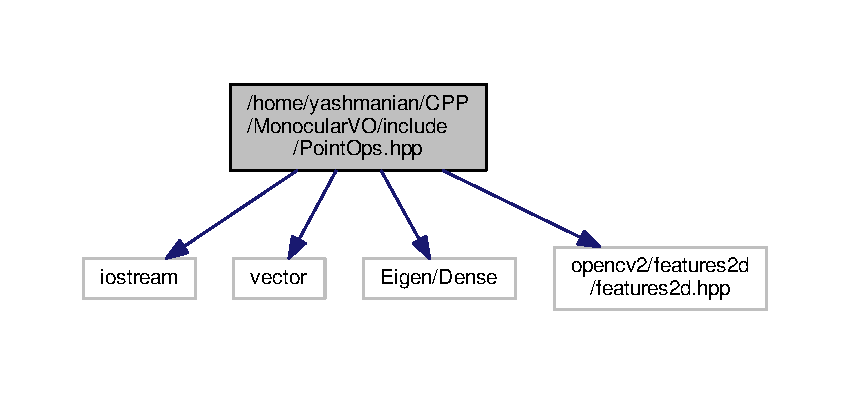
\includegraphics[width=350pt]{_point_ops_8hpp__incl}
\end{center}
\end{figure}
This graph shows which files directly or indirectly include this file\+:\nopagebreak
\begin{figure}[H]
\begin{center}
\leavevmode
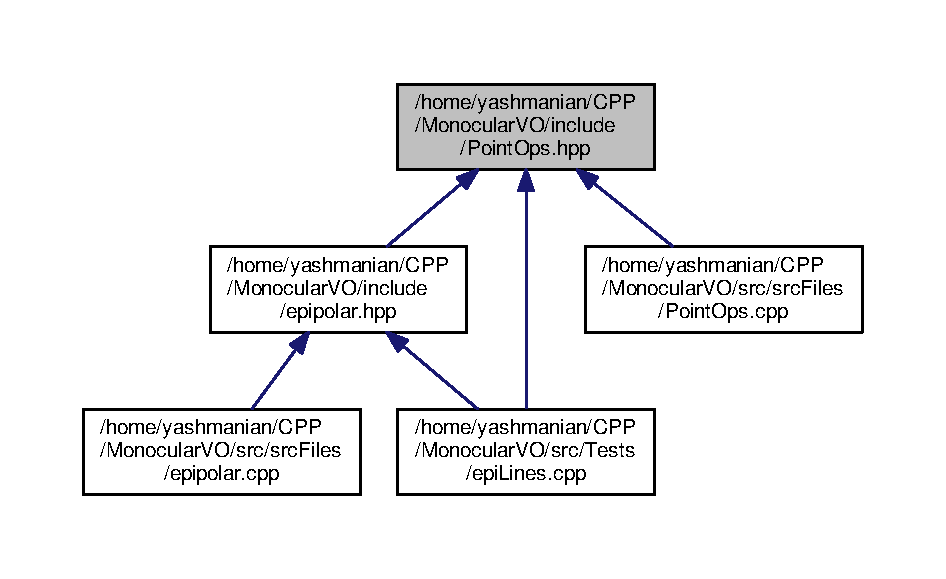
\includegraphics[width=350pt]{_point_ops_8hpp__dep__incl}
\end{center}
\end{figure}
\subsection*{Classes}
\begin{DoxyCompactItemize}
\item 
class \hyperlink{class_point_ops}{Point\+Ops}
\begin{DoxyCompactList}\small\item\em Definition of the \hyperlink{class_point_ops}{Point\+Ops} class. It contains all the functions and variables required manipulate point formats. \end{DoxyCompactList}\end{DoxyCompactItemize}


\subsection{Detailed Description}
Header file with definitions for class \hyperlink{class_point_ops}{Point\+Ops}. 

M\+IT License Copyright (c) 2018 Yash Manian Permission is hereby granted, free of charge, to any person obtaining a copy of this software and associated documentation files (the \char`\"{}\+Software\char`\"{}), to deal in the Software without restriction, including without limitation the rights to use, copy, modify, merge, publish, distribute, sublicense, and/or sell copies of the Software, and to permit persons to whom the Software is furnished to do so, subject to the following conditions\+: The above copyright notice and this permission notice shall be included in all copies or substantial portions of the Software. T\+HE S\+O\+F\+T\+W\+A\+RE IS P\+R\+O\+V\+I\+D\+ED \char`\"{}\+A\+S I\+S\char`\"{}, W\+I\+T\+H\+O\+UT W\+A\+R\+R\+A\+N\+TY OF A\+NY K\+I\+ND, E\+X\+P\+R\+E\+SS OR I\+M\+P\+L\+I\+ED, I\+N\+C\+L\+U\+D\+I\+NG B\+UT N\+OT L\+I\+M\+I\+T\+ED TO T\+HE W\+A\+R\+R\+A\+N\+T\+I\+ES OF M\+E\+R\+C\+H\+A\+N\+T\+A\+B\+I\+L\+I\+TY, F\+I\+T\+N\+E\+SS F\+OR A P\+A\+R\+T\+I\+C\+U\+L\+AR P\+U\+R\+P\+O\+SE A\+ND N\+O\+N\+I\+N\+F\+R\+I\+N\+G\+E\+M\+E\+NT. IN NO E\+V\+E\+NT S\+H\+A\+LL T\+HE A\+U\+T\+H\+O\+RS OR C\+O\+P\+Y\+R\+I\+G\+HT H\+O\+L\+D\+E\+RS BE L\+I\+A\+B\+LE F\+OR A\+NY C\+L\+A\+IM, D\+A\+M\+A\+G\+ES OR O\+T\+H\+ER L\+I\+A\+B\+I\+L\+I\+TY, W\+H\+E\+T\+H\+ER IN AN A\+C\+T\+I\+ON OF C\+O\+N\+T\+R\+A\+CT, T\+O\+RT OR O\+T\+H\+E\+R\+W\+I\+SE, A\+R\+I\+S\+I\+NG F\+R\+OM, O\+UT OF OR IN C\+O\+N\+N\+E\+C\+T\+I\+ON W\+I\+TH T\+HE S\+O\+F\+T\+W\+A\+RE OR T\+HE U\+SE OR O\+T\+H\+ER D\+E\+A\+L\+I\+N\+GS IN T\+HE S\+O\+F\+T\+W\+A\+RE.

\begin{DoxyCopyright}{Copyright}
Copyright 2018 Yash Manian
\end{DoxyCopyright}
\begin{DoxyAuthor}{Author}
Yash Manian Declaration of methods to manipulate point formats. 
\end{DoxyAuthor}

\hypertarget{epipolar_8cpp}{}\section{/home/yashmanian/\+C\+P\+P/\+Monocular\+V\+O/src/src\+Files/epipolar.cpp File Reference}
\label{epipolar_8cpp}\index{/home/yashmanian/\+C\+P\+P/\+Monocular\+V\+O/src/src\+Files/epipolar.\+cpp@{/home/yashmanian/\+C\+P\+P/\+Monocular\+V\+O/src/src\+Files/epipolar.\+cpp}}


Function definitions for methods declared in class epipolar.  


{\ttfamily \#include \char`\"{}epipolar.\+hpp\char`\"{}}\\*
Include dependency graph for epipolar.\+cpp\+:\nopagebreak
\begin{figure}[H]
\begin{center}
\leavevmode
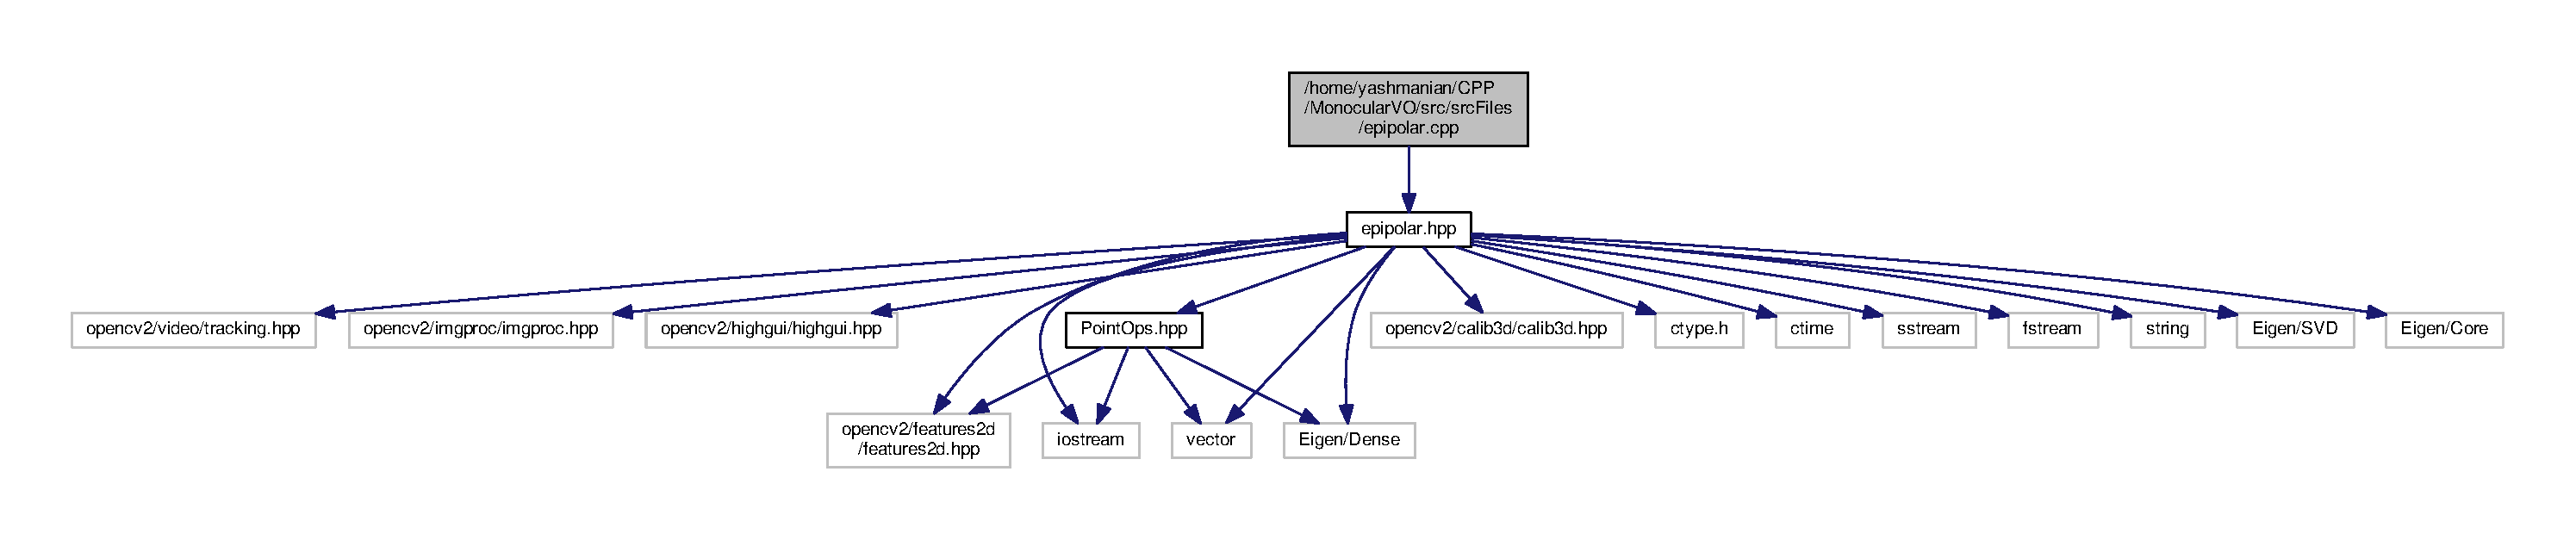
\includegraphics[width=350pt]{epipolar_8cpp__incl}
\end{center}
\end{figure}


\subsection{Detailed Description}
Function definitions for methods declared in class epipolar. 

M\+IT License Copyright (c) 2018 Yash Manian Permission is hereby granted, free of charge, to any person obtaining a copy of this software and associated documentation files (the \char`\"{}\+Software\char`\"{}), to deal in the Software without restriction, including without limitation the rights to use, copy, modify, merge, publish, distribute, sublicense, and/or sell copies of the Software, and to permit persons to whom the Software is furnished to do so, subject to the following conditions\+: The above copyright notice and this permission notice shall be included in all copies or substantial portions of the Software. T\+HE S\+O\+F\+T\+W\+A\+RE IS P\+R\+O\+V\+I\+D\+ED \char`\"{}\+A\+S I\+S\char`\"{}, W\+I\+T\+H\+O\+UT W\+A\+R\+R\+A\+N\+TY OF A\+NY K\+I\+ND, E\+X\+P\+R\+E\+SS OR I\+M\+P\+L\+I\+ED, I\+N\+C\+L\+U\+D\+I\+NG B\+UT N\+OT L\+I\+M\+I\+T\+ED TO T\+HE W\+A\+R\+R\+A\+N\+T\+I\+ES OF M\+E\+R\+C\+H\+A\+N\+T\+A\+B\+I\+L\+I\+TY, F\+I\+T\+N\+E\+SS F\+OR A P\+A\+R\+T\+I\+C\+U\+L\+AR P\+U\+R\+P\+O\+SE A\+ND N\+O\+N\+I\+N\+F\+R\+I\+N\+G\+E\+M\+E\+NT. IN NO E\+V\+E\+NT S\+H\+A\+LL T\+HE A\+U\+T\+H\+O\+RS OR C\+O\+P\+Y\+R\+I\+G\+HT H\+O\+L\+D\+E\+RS BE L\+I\+A\+B\+LE F\+OR A\+NY C\+L\+A\+IM, D\+A\+M\+A\+G\+ES OR O\+T\+H\+ER L\+I\+A\+B\+I\+L\+I\+TY, W\+H\+E\+T\+H\+ER IN AN A\+C\+T\+I\+ON OF C\+O\+N\+T\+R\+A\+CT, T\+O\+RT OR O\+T\+H\+E\+R\+W\+I\+SE, A\+R\+I\+S\+I\+NG F\+R\+OM, O\+UT OF OR IN C\+O\+N\+N\+E\+C\+T\+I\+ON W\+I\+TH T\+HE S\+O\+F\+T\+W\+A\+RE OR T\+HE U\+SE OR O\+T\+H\+ER D\+E\+A\+L\+I\+N\+GS IN T\+HE S\+O\+F\+T\+W\+A\+RE.

\begin{DoxyCopyright}{Copyright}
Copyright 2018 Yash Manian
\end{DoxyCopyright}
\begin{DoxyAuthor}{Author}
Yash Manian The following is a collection of methods to compute various Epipolar constraints 
\end{DoxyAuthor}

\hypertarget{_feat_track_8cpp}{}\section{/home/yashmanian/\+C\+P\+P/\+Monocular\+V\+O/src/src\+Files/\+Feat\+Track.cpp File Reference}
\label{_feat_track_8cpp}\index{/home/yashmanian/\+C\+P\+P/\+Monocular\+V\+O/src/src\+Files/\+Feat\+Track.\+cpp@{/home/yashmanian/\+C\+P\+P/\+Monocular\+V\+O/src/src\+Files/\+Feat\+Track.\+cpp}}


Function definitions for methods declared in class \hyperlink{class_feat_track}{Feat\+Track}.  


{\ttfamily \#include \char`\"{}Feat\+Track.\+hpp\char`\"{}}\\*
Include dependency graph for Feat\+Track.\+cpp\+:
\nopagebreak
\begin{figure}[H]
\begin{center}
\leavevmode
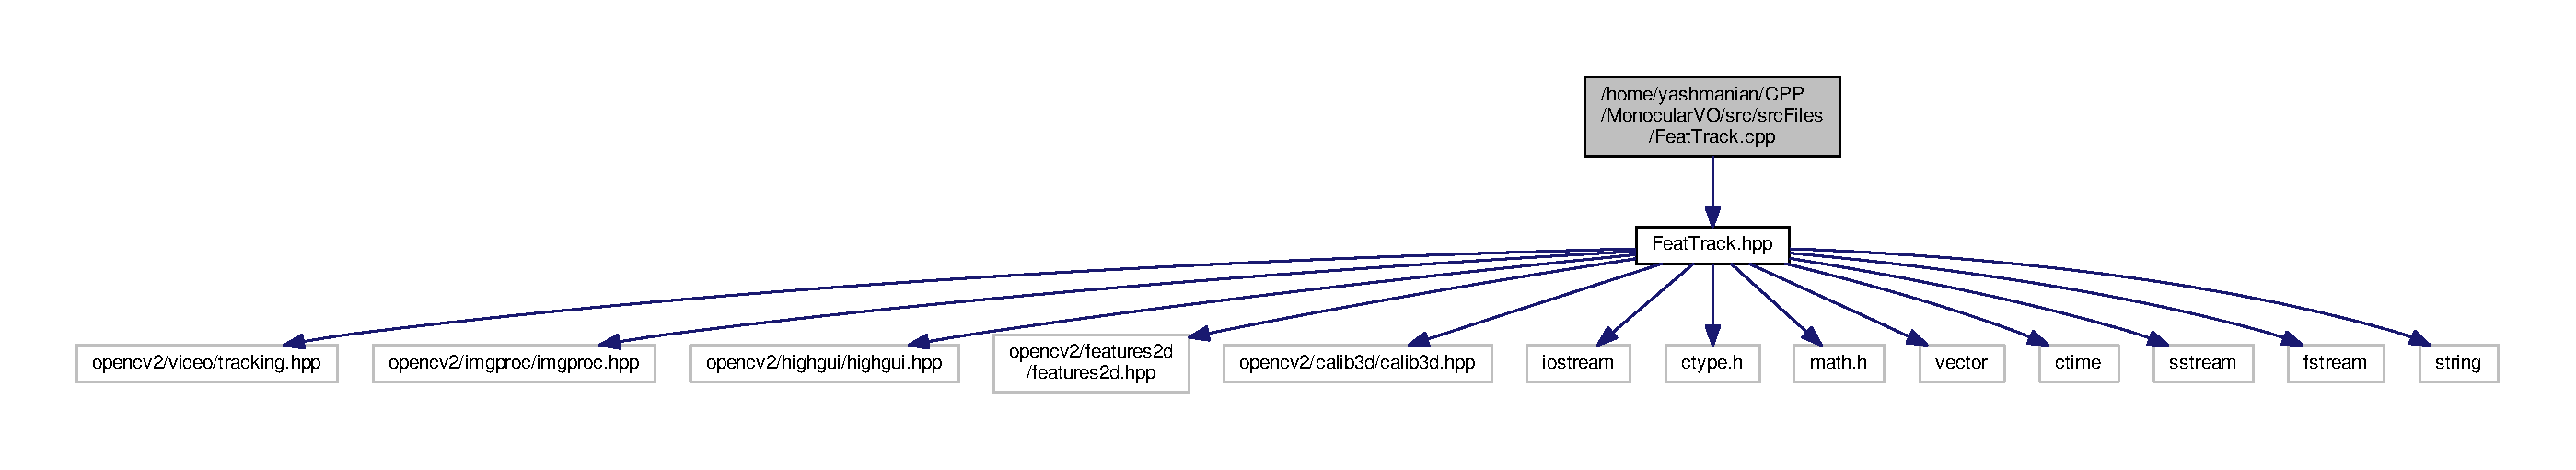
\includegraphics[width=350pt]{_feat_track_8cpp__incl}
\end{center}
\end{figure}


\subsection{Detailed Description}
Function definitions for methods declared in class \hyperlink{class_feat_track}{Feat\+Track}. 

M\+IT License Copyright (c) 2018 Yash Manian Permission is hereby granted, free of charge, to any person obtaining a copy of this software and associated documentation files (the \char`\"{}\+Software\char`\"{}), to deal in the Software without restriction, including without limitation the rights to use, copy, modify, merge, publish, distribute, sublicense, and/or sell copies of the Software, and to permit persons to whom the Software is furnished to do so, subject to the following conditions\+: The above copyright notice and this permission notice shall be included in all copies or substantial portions of the Software. T\+HE S\+O\+F\+T\+W\+A\+RE IS P\+R\+O\+V\+I\+D\+ED \char`\"{}\+A\+S I\+S\char`\"{}, W\+I\+T\+H\+O\+UT W\+A\+R\+R\+A\+N\+TY OF A\+NY K\+I\+ND, E\+X\+P\+R\+E\+SS OR I\+M\+P\+L\+I\+ED, I\+N\+C\+L\+U\+D\+I\+NG B\+UT N\+OT L\+I\+M\+I\+T\+ED TO T\+HE W\+A\+R\+R\+A\+N\+T\+I\+ES OF M\+E\+R\+C\+H\+A\+N\+T\+A\+B\+I\+L\+I\+TY, F\+I\+T\+N\+E\+SS F\+OR A P\+A\+R\+T\+I\+C\+U\+L\+AR P\+U\+R\+P\+O\+SE A\+ND N\+O\+N\+I\+N\+F\+R\+I\+N\+G\+E\+M\+E\+NT. IN NO E\+V\+E\+NT S\+H\+A\+LL T\+HE A\+U\+T\+H\+O\+RS OR C\+O\+P\+Y\+R\+I\+G\+HT H\+O\+L\+D\+E\+RS BE L\+I\+A\+B\+LE F\+OR A\+NY C\+L\+A\+IM, D\+A\+M\+A\+G\+ES OR O\+T\+H\+ER L\+I\+A\+B\+I\+L\+I\+TY, W\+H\+E\+T\+H\+ER IN AN A\+C\+T\+I\+ON OF C\+O\+N\+T\+R\+A\+CT, T\+O\+RT OR O\+T\+H\+E\+R\+W\+I\+SE, A\+R\+I\+S\+I\+NG F\+R\+OM, O\+UT OF OR IN C\+O\+N\+N\+E\+C\+T\+I\+ON W\+I\+TH T\+HE S\+O\+F\+T\+W\+A\+RE OR T\+HE U\+SE OR O\+T\+H\+ER D\+E\+A\+L\+I\+N\+GS IN T\+HE S\+O\+F\+T\+W\+A\+RE.

\begin{DoxyCopyright}{Copyright}
Copyright 2018 Yash Manian
\end{DoxyCopyright}
\begin{DoxyAuthor}{Author}
Yash Manian The following is a collection of methods to detect, track and compute homography 
\end{DoxyAuthor}

\hypertarget{_point_ops_8cpp}{}\section{/home/yashmanian/\+C\+P\+P/\+Monocular\+V\+O/src/src\+Files/\+Point\+Ops.cpp File Reference}
\label{_point_ops_8cpp}\index{/home/yashmanian/\+C\+P\+P/\+Monocular\+V\+O/src/src\+Files/\+Point\+Ops.\+cpp@{/home/yashmanian/\+C\+P\+P/\+Monocular\+V\+O/src/src\+Files/\+Point\+Ops.\+cpp}}


Function definitions for methods declared in class \hyperlink{class_point_ops}{Point\+Ops}.  


{\ttfamily \#include \char`\"{}Point\+Ops.\+hpp\char`\"{}}\\*
Include dependency graph for Point\+Ops.\+cpp\+:\nopagebreak
\begin{figure}[H]
\begin{center}
\leavevmode
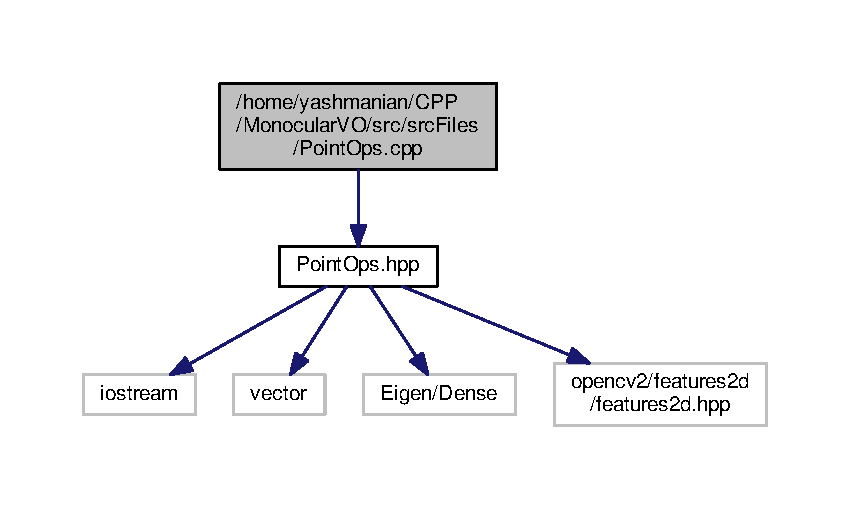
\includegraphics[width=350pt]{_point_ops_8cpp__incl}
\end{center}
\end{figure}


\subsection{Detailed Description}
Function definitions for methods declared in class \hyperlink{class_point_ops}{Point\+Ops}. 

M\+IT License Copyright (c) 2018 Yash Manian Permission is hereby granted, free of charge, to any person obtaining a copy of this software and associated documentation files (the \char`\"{}\+Software\char`\"{}), to deal in the Software without restriction, including without limitation the rights to use, copy, modify, merge, publish, distribute, sublicense, and/or sell copies of the Software, and to permit persons to whom the Software is furnished to do so, subject to the following conditions\+: The above copyright notice and this permission notice shall be included in all copies or substantial portions of the Software. T\+HE S\+O\+F\+T\+W\+A\+RE IS P\+R\+O\+V\+I\+D\+ED \char`\"{}\+A\+S I\+S\char`\"{}, W\+I\+T\+H\+O\+UT W\+A\+R\+R\+A\+N\+TY OF A\+NY K\+I\+ND, E\+X\+P\+R\+E\+SS OR I\+M\+P\+L\+I\+ED, I\+N\+C\+L\+U\+D\+I\+NG B\+UT N\+OT L\+I\+M\+I\+T\+ED TO T\+HE W\+A\+R\+R\+A\+N\+T\+I\+ES OF M\+E\+R\+C\+H\+A\+N\+T\+A\+B\+I\+L\+I\+TY, F\+I\+T\+N\+E\+SS F\+OR A P\+A\+R\+T\+I\+C\+U\+L\+AR P\+U\+R\+P\+O\+SE A\+ND N\+O\+N\+I\+N\+F\+R\+I\+N\+G\+E\+M\+E\+NT. IN NO E\+V\+E\+NT S\+H\+A\+LL T\+HE A\+U\+T\+H\+O\+RS OR C\+O\+P\+Y\+R\+I\+G\+HT H\+O\+L\+D\+E\+RS BE L\+I\+A\+B\+LE F\+OR A\+NY C\+L\+A\+IM, D\+A\+M\+A\+G\+ES OR O\+T\+H\+ER L\+I\+A\+B\+I\+L\+I\+TY, W\+H\+E\+T\+H\+ER IN AN A\+C\+T\+I\+ON OF C\+O\+N\+T\+R\+A\+CT, T\+O\+RT OR O\+T\+H\+E\+R\+W\+I\+SE, A\+R\+I\+S\+I\+NG F\+R\+OM, O\+UT OF OR IN C\+O\+N\+N\+E\+C\+T\+I\+ON W\+I\+TH T\+HE S\+O\+F\+T\+W\+A\+RE OR T\+HE U\+SE OR O\+T\+H\+ER D\+E\+A\+L\+I\+N\+GS IN T\+HE S\+O\+F\+T\+W\+A\+RE.

\begin{DoxyCopyright}{Copyright}
Copyright 2018 Yash Manian
\end{DoxyCopyright}
\begin{DoxyAuthor}{Author}
Yash Manian The following is a collection of methods to manipulate point formats. 
\end{DoxyAuthor}

\hypertarget{epi_lines_8cpp}{}\section{/home/yashmanian/\+C\+P\+P/\+Monocular\+V\+O/src/\+Tests/epi\+Lines.cpp File Reference}
\label{epi_lines_8cpp}\index{/home/yashmanian/\+C\+P\+P/\+Monocular\+V\+O/src/\+Tests/epi\+Lines.\+cpp@{/home/yashmanian/\+C\+P\+P/\+Monocular\+V\+O/src/\+Tests/epi\+Lines.\+cpp}}


File to compute epipolar lines and verify position of epipole.  


{\ttfamily \#include \char`\"{}Feat\+Track.\+hpp\char`\"{}}\\*
{\ttfamily \#include \char`\"{}epipolar.\+hpp\char`\"{}}\\*
{\ttfamily \#include \char`\"{}Point\+Ops.\+hpp\char`\"{}}\\*
{\ttfamily \#include $<$ctime$>$}\\*
Include dependency graph for epi\+Lines.\+cpp\+:\nopagebreak
\begin{figure}[H]
\begin{center}
\leavevmode
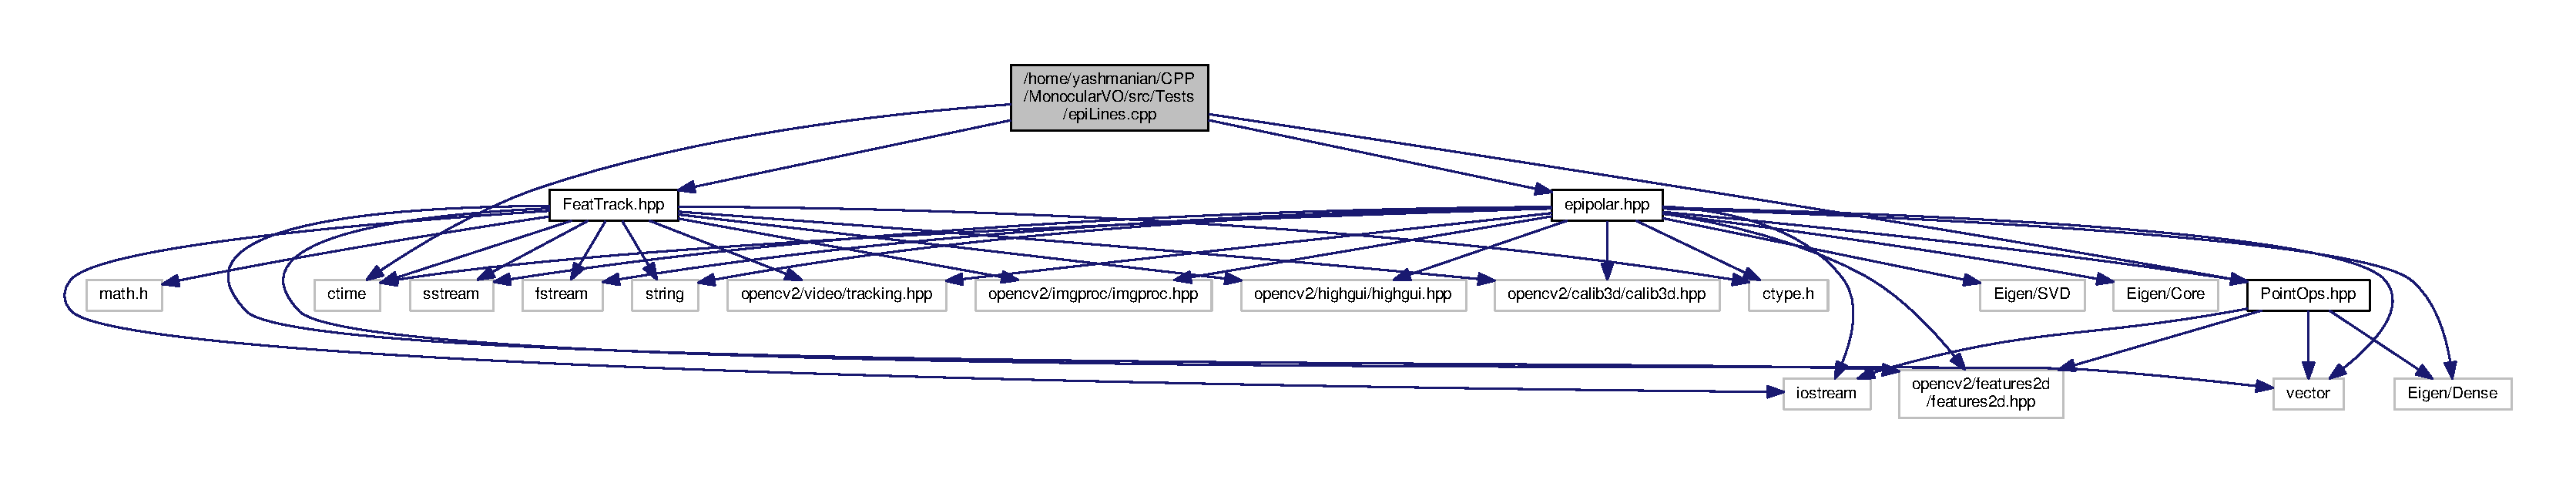
\includegraphics[width=350pt]{epi_lines_8cpp__incl}
\end{center}
\end{figure}
\subsection*{Functions}
\begin{DoxyCompactItemize}
\item 
int {\bfseries main} ()\hypertarget{epi_lines_8cpp_ae66f6b31b5ad750f1fe042a706a4e3d4}{}\label{epi_lines_8cpp_ae66f6b31b5ad750f1fe042a706a4e3d4}

\end{DoxyCompactItemize}


\subsection{Detailed Description}
File to compute epipolar lines and verify position of epipole. 

M\+IT License Copyright (c) 2018 Yash Manian Permission is hereby granted, free of charge, to any person obtaining a copy of this software and associated documentation files (the \char`\"{}\+Software\char`\"{}), to deal in the Software without restriction, including without limitation the rights to use, copy, modify, merge, publish, distribute, sublicense, and/or sell copies of the Software, and to permit persons to whom the Software is furnished to do so, subject to the following conditions\+: The above copyright notice and this permission notice shall be included in all copies or substantial portions of the Software. T\+HE S\+O\+F\+T\+W\+A\+RE IS P\+R\+O\+V\+I\+D\+ED \char`\"{}\+A\+S I\+S\char`\"{}, W\+I\+T\+H\+O\+UT W\+A\+R\+R\+A\+N\+TY OF A\+NY K\+I\+ND, E\+X\+P\+R\+E\+SS OR I\+M\+P\+L\+I\+ED, I\+N\+C\+L\+U\+D\+I\+NG B\+UT N\+OT L\+I\+M\+I\+T\+ED TO T\+HE W\+A\+R\+R\+A\+N\+T\+I\+ES OF M\+E\+R\+C\+H\+A\+N\+T\+A\+B\+I\+L\+I\+TY, F\+I\+T\+N\+E\+SS F\+OR A P\+A\+R\+T\+I\+C\+U\+L\+AR P\+U\+R\+P\+O\+SE A\+ND N\+O\+N\+I\+N\+F\+R\+I\+N\+G\+E\+M\+E\+NT. IN NO E\+V\+E\+NT S\+H\+A\+LL T\+HE A\+U\+T\+H\+O\+RS OR C\+O\+P\+Y\+R\+I\+G\+HT H\+O\+L\+D\+E\+RS BE L\+I\+A\+B\+LE F\+OR A\+NY C\+L\+A\+IM, D\+A\+M\+A\+G\+ES OR O\+T\+H\+ER L\+I\+A\+B\+I\+L\+I\+TY, W\+H\+E\+T\+H\+ER IN AN A\+C\+T\+I\+ON OF C\+O\+N\+T\+R\+A\+CT, T\+O\+RT OR O\+T\+H\+E\+R\+W\+I\+SE, A\+R\+I\+S\+I\+NG F\+R\+OM, O\+UT OF OR IN C\+O\+N\+N\+E\+C\+T\+I\+ON W\+I\+TH T\+HE S\+O\+F\+T\+W\+A\+RE OR T\+HE U\+SE OR O\+T\+H\+ER D\+E\+A\+L\+I\+N\+GS IN T\+HE S\+O\+F\+T\+W\+A\+RE.

\begin{DoxyCopyright}{Copyright}
Copyright 2018 Yash Manian
\end{DoxyCopyright}
\begin{DoxyAuthor}{Author}
Yash Manian 
\end{DoxyAuthor}

%--- End generated contents ---

% Index
\backmatter
\newpage
\phantomsection
\clearemptydoublepage
\addcontentsline{toc}{chapter}{Index}
\printindex

\end{document}
